% Clast de documento
\documentclass[12pt, letterpaper]{article}

% Paquetes
\usepackage[utf8]{inputenc}
\usepackage[spanish]{babel}
\usepackage{biblatex}
\usepackage{csquotes}
\usepackage{graphicx}
\usepackage{datetime}
\usepackage{lipsum}
\usepackage{hyperref}
\usepackage{fancyhdr}
\usepackage{parskip}
\usepackage{amsmath}
\usepackage{listings}
\usepackage[table,xcdraw]{xcolor}
\usepackage{booktabs}

%------------ 
% Decoración
%------------

% Configuración de colores de python
\lstset{
    language=Python,
    basicstyle=\ttfamily\small,
    keywordstyle=\color{blue},
    commentstyle=\color{green},
    stringstyle=\color{red},
    showstringspaces=false,
    numbers=left,
    numberstyle=\tiny\color{gray},
    frame=single,
    breaklines=true
}

\lstset{
    literate={á}{{\'a}}1 {é}{{\'e}}1 {í}{{\'\i}}1 {ó}{{\'o}}1 {ú}{{\'u}}1
             {Á}{{\'A}}1 {É}{{\'E}}1 {Í}{{\'I}}1 {Ó}{{\'O}}1 {Ú}{{\'U}}1
             {ñ}{{\~n}}1 {Ñ}{{\~N}}1
             {¡}{{!`}}1 {¿}{{?`}}1 % Añade caracteres especiales en español
}

% Configuración de header y footer
\fancyhf{}
\setlength{\headheight}{15.71667pt}
\addtolength{\topmargin}{-3.71667pt}
\fancyhf{}

% Header
\fancyhead[L]{\textsc{\doctitle}}
\renewcommand{\sectionmark}[1]{\markright{#1}}
\fancyhead[R]{\textit{\nouppercase{\rightmark}}}

% Footer
\renewcommand{\footrulewidth}{0.4pt}
\fancyfoot[C]{Página \thepage}

% Título
\newcommand{\doctitle}{Ejercicios práctica 1}
\title{\doctitle}
\author{Juan Luis Serradilla Tormos}
\date{\monthname[\month] de \the\year}

% Bibliografía
\addbibresource{test.bib}

% Eliminar sangría
\setlength{\parindent}{0pt}

% Aumentar la separación entre párrafos
\setlength{\parskip}{1em plus 0.5em minus 0.2em}


%-----------
% Documento
%-----------
\begin{document}

% Mostrar header y footer
\pagestyle{fancy}

% Mostrar el título
\maketitle

% Índice
\newpage
\tableofcontents

% Contenido
\newpage
\section{Ejercicio 1.5.3}
\textbf{Una tienda de abarrotes recibe su suministro semanal de
huevos cada jueves por la mañana. Este envío debe durar hasta el jueves
siguiente, cuando llega un nuevo pedido. Cualquier huevo no vendido antes
del jueves se descarta. Los huevos se venden a \$10 por cada cien y cuestan
\$8 por cada cien. La demanda semanal de huevos en esta tienda variaba de una
semana a otra. Basándose en la experiencia pasada, se asigna la siguiente
distribución de probabilidad a la demanda semanal:}
\begin{table}[h]
    \centering
    \begin{tabular}{cccccc}
        \toprule
        \textbf{Demanda (x100 huevos)} & 10 & 11 & 12 & 13 & 14 \\
        \midrule
        \textbf{Probabilidad de demanda} & 0.1 & 0.2 & 0.4 & 0.2 & 0.1 \\
        \bottomrule
    \end{tabular}
\end{table}
\textbf{Este patrón de demanda se mantiene estable durante todo el año; la
demanda de huevos no es estacional y la tendencia es plana. El problema
es: ¿Cuántos huevos deben ordenarse para la entrega cada jueves?}

Para poder ver cuántos huevos se deben ordenar lo primero que hay que hacer es determinar una función beneficio.
\begin{align*}
    & n \equiv \text{Número de huevos ordenados} \\ 
    & d \equiv \text{Demanda semanal} \\
    & p \equiv \text{probabilidad de demanda} \\
    & c \equiv \text{Costo de los huevos} \\
    & v \equiv \text{Valor de los huevos} 
\end{align*}

La variable $d_i$ representa la demanda semanal de la semana $i$, $p_i$ la probabilidad de que ocurra dicha demanda y $n_j$  la cantidad de huevos que se encargan, tal que $i,j \in \{1,2,3,4,5\}$. La cantidad de huevos que se encargan oscilan entre los valores de $d$ ya que si se piden menos del $\min{d}$ se perderán ventas y si se piden más del $\max{d}$ se dejarán huevos sin vender. Por tanto, la función beneficio se puede expresar como:
\[
    B(n_j,d_i) = \begin{cases}
        n_j \cdot (v - c) & \text{si } j \leq i \\
        d_i \cdot v - n_j \cdot c & \text{si } j > i
    \end{cases}
\]

\newpage
Ahora que tenemos la función beneficio, tenemos que calcular el beneficio medio para una cantidad $n_j$. Para ello, se calcula el beneficio medio ponderado por la probabilidad de que ocurra una demanda $d_i$:
\[
    \bar{B}(n_j) = \sum_{i=1}^{5} p_i \cdot B(n_j,d_i) = 
    \sum_{i<j}p_i(d_i \cdot v - n_j \cdot c) + \sum_{i \geq j}p_i(n_j \cdot (v - c))
\]

Reordenando y juntando términos, se obtiene:
\[
    \bar{B}(n_j) = 
        v\sum_{i<j}p_i d_i + 
        v n_j \sum_{i \geq j} p_i -
        c n_j
\]

Ahora, vamos a aplicar la función beneficio a cada posible valor de $j$.
\begin{align*}
    & j = 1 \Rightarrow B(10) = 20 \\
    & j = 2 \Rightarrow B(11) = 21 \\
    & j = 3 \Rightarrow B(12) = 20 \\
    & j = 4 \Rightarrow B(13) = 15 \\
    & j = 5 \Rightarrow B(14) = 8
\end{align*}

Finalmente, vemos que el valor óptimo de $n$ es $n = 11$, que da un beneficio medio de 21\$.

\newpage
\section{Ejercicio 1.5.4}
\textbf{La función de utilidad de Ana es $U = \sqrt{w}$, donde $w$ es el
dinero. Ella es dueña de una panadería, la cual el año que viene puede valer
o bien 0 o bien 100 euros con las mismas posibilidades.}
\begin{enumerate}
    \item \textbf{Supongamos que su empresa es el único activo que posee. ¿Cuál es el precio P más bajo al que aceptaría vender su panadería?}

    La función de utilidad es $U = \sqrt{w}$, por lo que la utilidad media es $\bar{U} = \sum_i p_i\sqrt{w_i}$. Sustituyendo tenemos $\bar{U} = \frac{1}{2}(\sqrt{0} + \sqrt{100}) = \frac{1}{2}(0 + 10) = 5$. 

    Ahora que tenemos la utilidad media, si despejamos el precio medio como $\bar{w} = \bar{U}^2$ obtenemos que $\bar{w} = 5^2 = 25$. Por tanto, el precio más bajo al que aceptaría vender su panadería es 25 euros.

    \item \textbf{Supongamos que tiene tiene 100 euros guardados ¿Cómo afectaría en este caso al caso anterior?}
    
    En este caso tenemos que $\bar{U} = \sum_i p_i\sqrt{100 + w_i}$, por lo que sustotuyendo tenemos $\bar{U} = \frac{1}{2}(\sqrt{100 + 0} + \sqrt{100 + 100}) = \frac{1}{2}(10 + 14.14) = 12.07$. 

    Si despejamos la utilidad media como $\bar{w} = \bar{U}^2 - 100$ obtenemos que $\bar{w} = 12.07^2 - 100 = 45.7$. Por tanto, el precio más bajo al que aceptaría vender su panadería es 45.7 euros.

    \item\textbf{Compara tus resultados de las partes anteriores. ¿Cuál es la relación entre los ingresos de Ana y su aversión al riesgo?}
    
    La aversión al riesgo se calcula como $A(w) = -\frac{d^2U}{dw^2} {\big(\frac{dU}{dw}\big)}^{-1}$. Calculando las derivadas tenemos:
    \begin{align*}
        &   \frac{dU}{dw} = \frac{1}{2\sqrt{w}},\
        \frac{d^2U}{dw^2} = -\frac{1}{4w\sqrt{w}} \Rightarrow
        A(w) = \frac{1}{2\sqrt{w}}
    \end{align*}

    Podemos ver que la aversión al riesgo disminuye cuando aumenta el dinero.

\end{enumerate}

\newpage

\section{Ejercicio 1.5.5}
\textbf{Resuelve el siguiente problema de decisión multiobjetivo. Describa el frente de pareto:}
\begin{align*}
    & \min f_1(x,y) = 2x^{2} - 5y + y^{2} \\
    & \max f_2(x,y) = x^{2} + 14x + 5y -74
\end{align*}
\textbf{sujeto a:}
\begin{align*}
    & x + y \geq 15, \\
    & x - y \leq 5, \\
    & 2x + y \geq 20, \\
    & 0 \leq x \leq 20, \\
    & 0 \leq y \leq 20
\end{align*}

Para poder visualizar el frente de Pareto lo primero que vamos a hacer es representar las funciones con Python. Como queremos minimizar la función $f_1$ vamos a representar $-f_1$, de forma que busquemos el máximo en las dos funciones. 

\begin{figure}[h]
    \centering
    \begin{minipage}{0.48\textwidth}
        \centering
        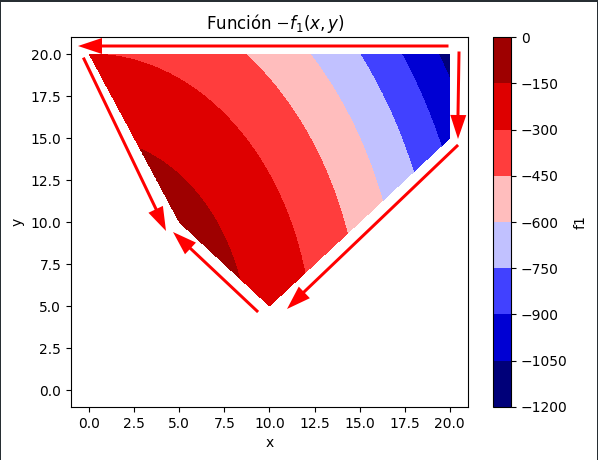
\includegraphics[width=\textwidth]{images/f1.png}
        \caption{Valor de la función $f_1$ dentro de la superficie\label{fig:f1}}
    \end{minipage}
    \hfill
    \begin{minipage}{0.48\textwidth}
        \centering
        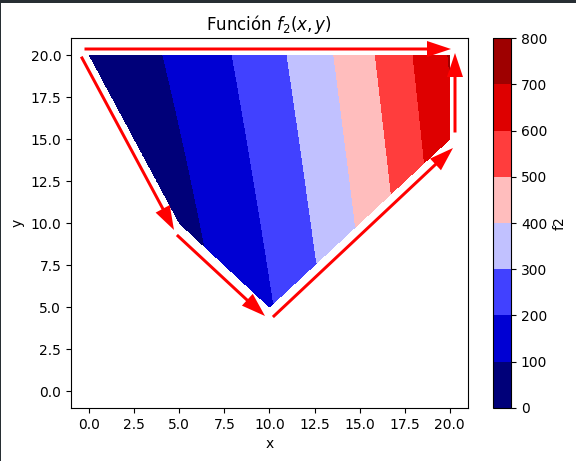
\includegraphics[width=\textwidth]{images/f2.png}
        \caption{Valor de la función $f_2$ dentro de la superficie\label{fig:f2}}
    \end{minipage}
\end{figure}

\newpage
Definimos el frente de Pareto los bordes donde si una solución mejora la otra empeora. Por tanto, si nos fijamos en las figuras~\ref{fig:f1} y~\ref{fig:f2} podemos ver que el frente de Pareto es el siguiente:

\begin{figure}[h]
    \centering
    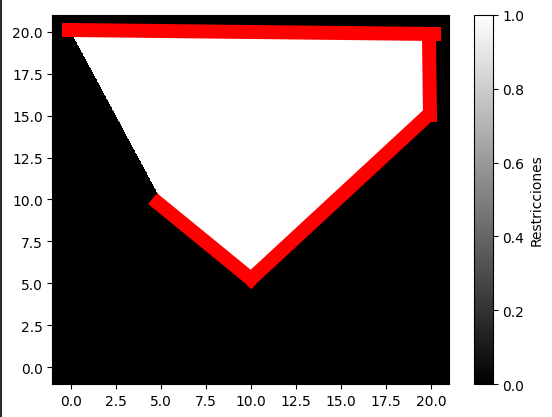
\includegraphics[width=10cm]{images/pareto.png}
    \caption{Frente de Pareto\label{fig:pareto}}
\end{figure}

Finalmente, para determinar el conjunto de soluciones óptimas vamos a hacer una ``media'' entre las dos funciones, de forma que transformemos el problema multiobjetivo en un problema de optimización único. Para ello, vamos a definir la función objetivo como:
\begin{align*}
    & f_3(x,y) = \frac{f_2(x,y)}{2} - \frac{f_1(x,y)}{2}
\end{align*}
Restamos la función $f_1$ a la función $f_2$ ya que vamos a encontrar el máximo de $f_3$, por lo que así pasamos de minimizar $f_1$ a maximizarla.

\newpage
El resultado que obtenemos es el siguiente:
\begin{figure}[h]
    \centering
    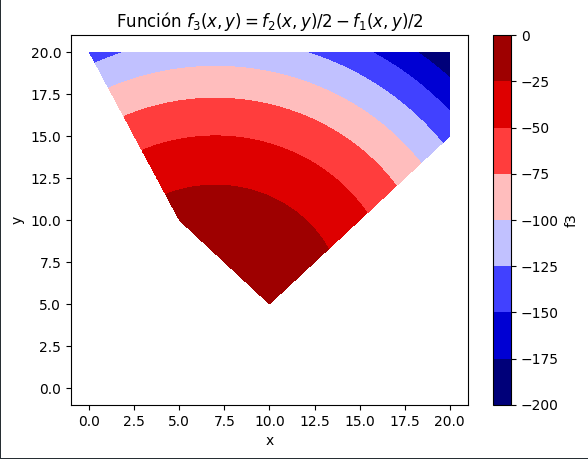
\includegraphics[width=10cm]{images/f3.png}
    \caption{Valor de la función $f_3$ dentro de la superficie\label{fig:f3}}
\end{figure}

Podemos observar como el el borde inferior-izquierdo es el que contiene los puntos máximos de la función, es decir, el que está entre $(10,5)$ y $(5,10)$. Si además utilizamos un script de Python para calcular el máximo de la función $f_3$, obtenemos que este máximo se encuentra en el punto $(x,y) = (8.49, 6.51)$.

\newpage

\section{Ejercicio 1.5.6}
\textbf{Eres el Científico de Datos de una importante empresa mayorista del sector turístico. La empresa tiene como negocio la creación de paquetes turísticos que luego vende a minoristas, agencias de viaje tanto online como offline. La empresa te pide lo siguiente:}

\textbf{Se ha realizado un estudio previo sobre toma de decisiones considerando los siguientes atributos y valores:}
\begin{itemize}
    \item \textbf{Calidad del paquete:} Número de estrellas del hotel (2, 3, 4 y 5).
    \item \textbf{Precio:} Valores comprendidos entre 120 y 870 euros.
    \item \textbf{Días del paquete:} 5 o 7.
    \item \textbf{Aspecto del producto:} Alta o Baja.
\end{itemize}

\textbf{Se elaboró un cuestionario que planteó 8 situaciones de elección, en cada una de las cuales se presentaron 3 paquetes turísticos. A los encuestados se les solicitó escoger el paquete más atractivo en cada situación.Tanto los atributos de cada situación de elección como los resultados de las elecciones para un conjunto de individuos se encuentran en un fichero Excel adjunto al boletín. Se pide crear un modelo que, dado un conjunto de 3 paquetes, prediga cuál será el más atractivo.}

Se ha leído el dataset de \texttt{paquetes.xlsx} y se ha transformado a un formato que pueda ser utilizado por el algoritmo de \textit{Random Forest}. Para ello, se ha utilizado la librería \texttt{pandas} de Python. El dataset es el siguiente:

\newpage
\begin{figure}[h]
    \centering
    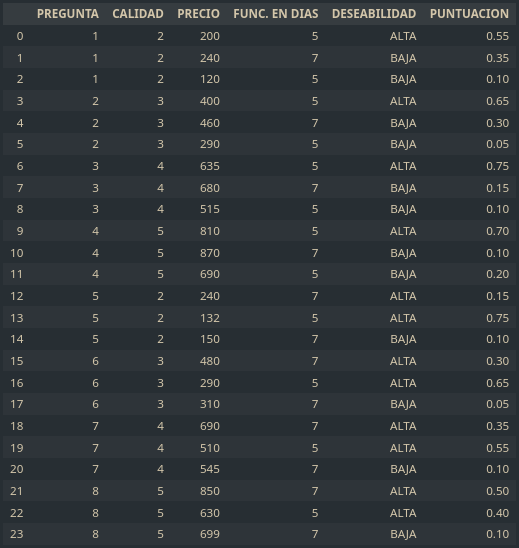
\includegraphics[width=10cm]{images/dataset.png}
    \caption{Dataset de paquetes turísticos\label{fig:paquetes}}
\end{figure}

\newpage
Se ha hecho un algoritmo de regresión de Random Forest con 100 árboles. La matriz de confusión del modelo es la siguiente:
\begin{figure}[h]
    \centering
    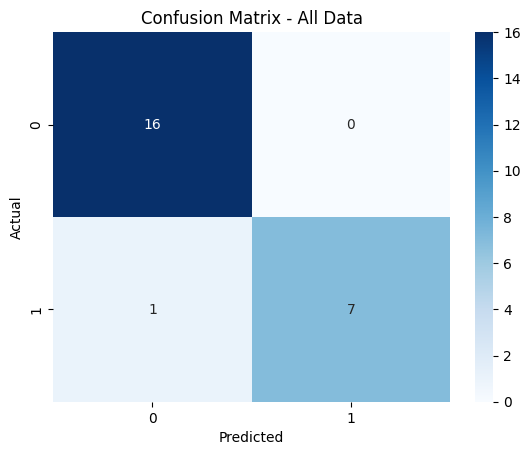
\includegraphics[width=10cm]{images/confusion_matrix.png}
    \caption{Matriz de confusión del modelo\label{fig:confusion_matrix}}
\end{figure}

\newpage
\section{Ejercicio 1.5.7}
\textbf{Obtener el equilibrio de Nash en estrategias mixtas del juego piedra, papel, tijera.}

Vamos a hacer una tabla con las ganancias de cada jugada en el piedra, papel, tijera. 
% Please add the following required packages to your document preamble:
% \usepackage[table,xcdraw]{xcolor}
% Beamer presentation requires \usepackage{colortbl} instead of \usepackage[table,xcdraw]{xcolor}
\begin{table}[h]
    \centering
    \begin{tabular}{c|c|c|c|}
    \cline{2-4}
     &
      \cellcolor[HTML]{000000}{\color[HTML]{FFFFFF} \textbf{PIEDRA}} &
      \cellcolor[HTML]{000000}{\color[HTML]{FFFFFF} \textbf{PAPEL}} &
      \cellcolor[HTML]{000000}{\color[HTML]{FFFFFF} \textbf{TIJERA}} \\ \hline
    \multicolumn{1}{|c|}{\cellcolor[HTML]{000000}{\color[HTML]{FFFFFF} \textbf{PIEDRA}}} & 0  & -1 & 1  \\ \hline
    \multicolumn{1}{|c|}{\cellcolor[HTML]{000000}{\color[HTML]{FFFFFF} \textbf{PAPEL}}}  & 1  & 0  & -1 \\ \hline
    \multicolumn{1}{|c|}{\cellcolor[HTML]{000000}{\color[HTML]{FFFFFF} \textbf{TIJERA}}} & -1 & 1  & 0  \\ \hline
    \end{tabular}
\end{table}

Podemos ver que en ``forma pura'' no hay equilibrio, ya que si una persona elige completamente una estrategia siempre hay otra estrategia que le gana. Por tanto, hay que utilizar estrategias mixtas, es decir, estrategias que otorgan probabilidades a las jugadas. Para ello asignamos las siguientes probabilidades:
\begin{align*}
    \text{Prob.\ roca}   \equiv p_{r} \qquad
    \text{Prob.\ papel}  \equiv p_{p} \qquad
    \text{Prob.\ tijera} \equiv p_{t}
\end{align*}
Hay que tener en cuenta la restricción $p_{r} + p_{p} + p_{t} = 1$. Ahora vemos las ganancias de cada jugada ($G_i$):
\begin{align*}
    & G_{r} = 0 \cdot p_{r} - 1 \cdot p_{p} + 1 \cdot p_{t} = p_{t} - p_{p} \\
    & G_{p} = 1 \cdot p_{r} + 0 \cdot p_{p} - 1 \cdot p_{t} = p_{r} - p_{t} \\
    & G_{t} = -1 \cdot p_{r} + 1 \cdot p_{p} + 0 \cdot p_{t} = p_{p} - p_{r}
\end{align*}

Ahora, hay que tener en cuenta que las ganancias deben ser las mismas ($G_{r} = G_{p} = G_{t}$). Por lo tanto, nos queda el siguiente sistema de ecuaciones:
\begin{align*}
    & 2*p_{t} = p_{r} + p_{p} \\
    & 2*p_{r} = p_{p} + p_{t} \\
    & 2*p_{p} = p_{r} + p_{t}
\end{align*}

Si resolvemos el sistema de ecuaciones obtenemos las siguientes probabilidades:
\begin{align*}
    p_{r} = \frac{1}{3} \qquad
    p_{p} = \frac{1}{3} \qquad
    p_{t} = \frac{1}{3}
\end{align*}

\end{document}
